\documentclass[a4paper, 12pt]{article}

\usepackage{hyperref}
\usepackage[warn]{mathtext}
\usepackage[utf8]{inputenc}
\usepackage[T2A]{fontenc}
\usepackage[english,russian]{babel}
\usepackage{multirow}
\usepackage{amsmath,amsfonts,amssymb,amsthm,mathtools}
\usepackage{indentfirst}
\DeclareSymbolFont{T2Aletters}{T2A}{cmr}{m}{it}
\usepackage{ gensymb }
\mathtoolsset{showonlyrefs=true}
\usepackage{euscript}
\usepackage{mathrsfs}
\usepackage[left=2cm,right=2cm,top=2cm,bottom=2cm]{geometry}
\usepackage{graphicx}
\usepackage{wrapfig}
\usepackage[rgb]{xcolor}
\hypersetup{
colorlinks=true,
urlcolor=blue
}


\title{Лабораторная работа 1.3.3}
\author{Гисич Арсений Б03-109}
\date{2022}

\begin{document}

	\begin{center}
		{\large МОСКОВСКИЙ ФИЗИКО-ТЕХНИЧЕСКИЙ ИНСТИТУТ (НАЦИОНАЛЬНЫЙ ИССЛЕДОВАТЕЛЬСКИЙ УНИВЕРСИТЕТ)}
	\end{center}
	\vspace{5 cm}
	{\Large
		\begin{center}
			{\bf Лабораторная работа 2.3.1А}\\[0.2 cm]
			Современные средства получения и измерения вакуума
		\end{center}
	}
	\vspace{4 cm}
	\begin{flushright}
		{\Large Выполнил: \\
			\vspace{0.2 cm}
			Гисич Арсений \\
			\vspace{0.2 cm}
			Б03-109 \\}
	\end{flushright}
	\vspace{9 cm}
	\begin{center}
		Долгопрудный\\[0.1 cm]
		2022
	\end{center}
\thispagestyle{empty}

\section{Аннотация}

\par Цель работы: определить откачиваемый объём и измерить скорость откачки форвакуумным насосом; измерить скорость откачки турбомолекулярным насосом и определить предельный вакуум; определить давление перехода в молекулярный режим; исследовать зависимость мощности турбонасоса от давления в камере.

\section{Теоретические сведения}

В физике вакуумом называют состояние газа, при котором характерная длина свободного пробега молекул в газе $\lambda$ сравнима по порядку
величины с характерным линейным размером сосуда $d$, в котором газ
находится. Для воздуха при нормальных условиях $\lambda \sim 10^{-5}~см$, откуда
видно, что воздух в жилых помещениях не находится в состоянии вакуума, но, например, внутри пористых материалов, таких как древесина, уже
может находиться.

В технике вакуумом называют состояние газа при котором его
давление меньше атмосферного ($P < P_{атм}$). Различают следующие типы
вакуума: \textit{низкий}, когда средняя длина свободного пробега молекул газа
значительно меньше характерного линейного размера рассматриваемого
объёма, т.е. $\lambda < d$; \textit{средний}, когда $\lambda \sim d$; \textit{высокий} (или глубокий), когда
$\lambda \gg d$ (рис. \ref{ris1}). Иногда выделяют ещё \textit{сверхвысокий} вакуум, при котором
не происходит заметного изменения свойств поверхности, первоначально
свободной от адсорбированного газа, за время, существенное
для проведения эксперимента. Газ в состоянии высокого вакуума называется \textit{ультраразреженным}.

\begin{figure}[h!]
	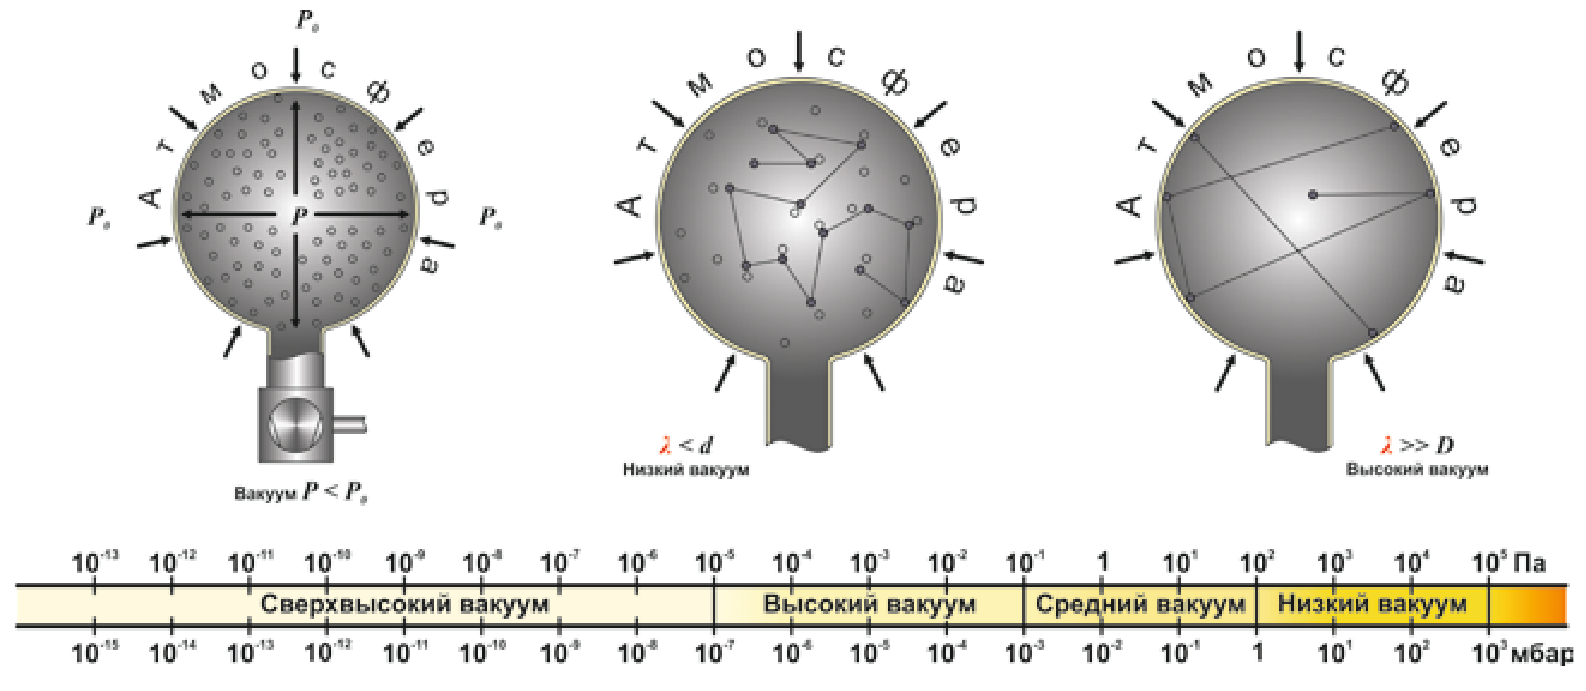
\includegraphics[width = \textwidth]{1.png}
\caption{Понятие о вкаууме}
\label{ris1}
\end{figure}

\subsection{Некоторые понятия для работы с вакуумной техникой}

Основы процесса откачки и связанные с ним понятия рассмотрим на примере простейшей вакуумной системы (рис. \ref{ris2}).

\begin{figure}[h!]
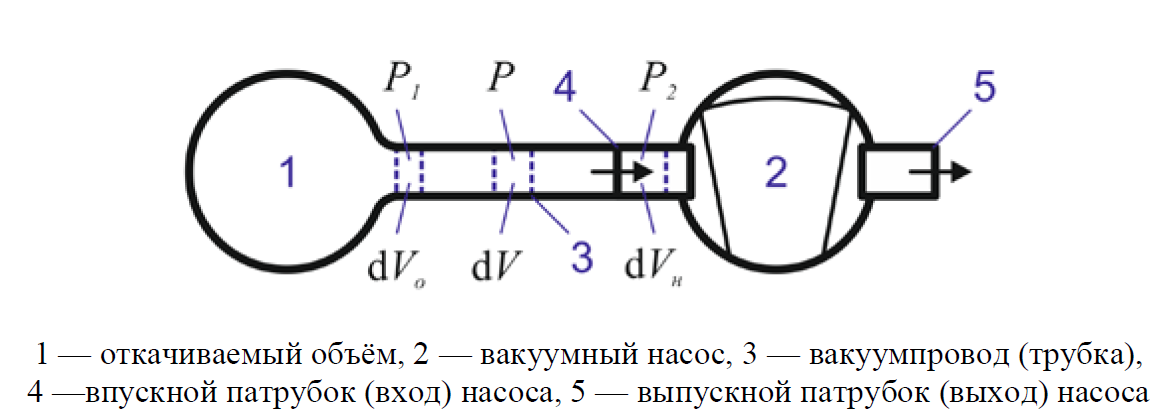
\includegraphics[width = \textwidth]{2.png}
\caption{Простейшая вакуумная система}
\label{ris2}
\end{figure}
Здесь и далее $L$ - единица измерения длины, $M$ - единица измерения массы, $T$ - единица измерения времени.
\begin{enumerate}
\item \textbf{Предельное остаточное давление} (предельный вакуум) $P_{\text{пр}} [L^{-1}MT^{-2}]$ -- наименьшее давление газа, которое формируется в процессе откачки в рассматриваемом сечении вакуумпровода (рассматриваемой точке вакуумной системы). Обычно выделяют предельное давление в камере или на входе в насос.
\item \textbf{Наибольшее выпускное давление} $[L^{-1}MT^{-2}]$ - максимально допустимое давление газа на входе насоса.
\item \textbf{Быстрота откачивающего действия} (скорость откачки) вакуумной системы $S [L^3T^{-1}]$ -- объем газа, проходящий через рассматриваемое сечение вакуумпровода в единицу времени при текущем давлении в данном сечении:
\[S = \dfrac{dV}{dT}.\]
Следовательно быстродействие насоса $S_{\text{н}}$ определяется как:
\[ S_{ \text{н} } = \dfrac{dV_{ \text{н} }}{ dt }.\]
А эффективная скорость откачки камеры $S_0$:
\[S_0 = \dfrac{ dV_0 }{ dt }.\]
\item Падение давления вдоль вакуумпровода $ \Delta P = P_1 - P_2 $ определяется его \textbf{пропускной способностью} (проводимостью) $ U [L^3 T^{-1} ] $:
\[ U = \dfrac{Q}{P_1 - P_2}, \]
где $Q [L^2 M T^{-3}]$ -- \textbf{поток газа} через вакуумпровод с соответствующими давлениями на концах.
\item Величина $Z [L^{-3}T]$, обратная проводимости, называется \textbf{импедансом} вакуумпровода:
\[Z=\dfrac{1}{U}.\]
В общем случае указанные величины $S$, $U$, $Q$, $Z$ как и сами давления $P_1$ и $P_2$ зависят от времени. Но в конце процесса откачки устанавливается квазистационарный режим, при котором поток газа становится практически постоянным и равным количеству поступающего в систему газа в единицу времени вследствие наличия течей, т.е. нарушения герметичности (в основном в местах механического соединения отдельных узлов вакуумной системы). Для стационарного режима можно записать условие непрерывности потока откачиваемого газа:
\[P_1 S_0 = PS = P_2 S_{\text{н}} = Q. \]
\item \textbf{Основное уравнение вакуумной техники}
\begin{equation}\label{main}
\dfrac{1}{S_0} = \dfrac{1}{S_{ \text{н} }} + \dfrac{1}{U}.
\end{equation}
\item Количественной характеристикой течи, является \textbf{натекание} $Q_н [L^2MT^{-3}]$, измеряемое при отключенных средствах откачки:
\[Q_н = \frac{P_к - P_н}{\Delta{t}},\]
где $V$ -- замкнутый исследуемый объём; $P_н, P_к$ -- начальное и конечное
давление в объеме; $\Delta{t}$ -- время между измерениями давления. При наличии течей, нормальной работе средств откачки и отсутствии в системе источников паров или газов, зависимость потока газа через течь от времени $Q_н(t)$ носит, как правило, линейный характер.

Для заданного давления $P_1$ в замкнутом исследуемом объёме допустимым считается натекание:
\[Q_н \ll Q = P_1S_0 = P_1\frac{S_нU}{S_н + U}.\]
\end{enumerate}

На пропускную способность вакуумпровода существенно влияет
режим течения газа, который характеризуется числом Кнудсена, равным
отношению длины свободного пробега молекул в газе к характерному
линейному размеру течения:
\[Kn = \dfrac{\lambda}{d}.\]
Данная величина характеризует степень разреженности газового
потока:
\begin{itemize}
\item В \textit{гидродинамическом} (вязкостном) режиме течения ($Kn \ll 1$)
различают ламинарные и турбулентные потоки. При ламинарном
течении молекулы газа движутся по параллельным траекториям
со скоростями, мало отличающимися друг от друга. При турбулентном течении наряду с поступательным движением всей массы газа, молекулы движутся хаотически со скоростями, подвергающимися случайным изменениям.
\item В \textit{молекулярном} (кнудсеновском) режиме ($Kn \gg 1$) течение газа
сводится к независимому движению отдельных молекул по прямым линиям в периоды между соударениями главным образом со
стенками вакуумпровода.
\item В \textit{переходном} режиме ($Kn \sim 1$) в системе могут существовать все
описанные выше виды течения.
\end{itemize}

В разных режимах течения пропускная способность вакуумпровода имеет существенно различные зависимости от размера его поперечного сечения.

\subsection{Проводимость отверстия в стенке}

В кнудсеновском режиме проводимость отверстия радиусом $R$ определяется средним числом молекул, сталкивающихся со стенкой:
\[\nu = \nu_2 - \nu_1 = \frac{1}{4}n_2\vartheta - \frac{1}{4}n_1\vartheta = \frac{1}{4}\frac{P_2}{kT}\vartheta - \frac{1}{4}\frac{P_1}{kT}\vartheta = \frac{1}{4}\frac{\vartheta}{kT}(P_2 - P_1),\]
с другой стороны:
\[\nu = \frac{1}{A}\left(\frac{dN_2}{dt} - \frac{dN_1}{dt}\right) = \frac{1}{A}\left(\frac{d(n_2V)}{dt} - \frac{d(n_1V}{dt}\right) = \frac{(n_2 - n_1)}{A}\frac{dV}{dt} =\]
\[= \frac{1}{A}\left(\frac{P_2}{kT} - \frac{P_1}{kT}\right)\frac{dV}{dt} = \frac{1}{AkT}(P_2 - P_1)U_{отв},\]
где $\nu$ -- число молекул пролетающих через единицу площади отверстия
за единицу времени, $A$ — площадь отверстия, $n$ -- концентрация молекул,
$\vartheta$ -- их средняя скорость, $T$ -- температура газа, $k$ -- постоянная Больцмана, индексы 2, 1 относятся к потокам молекул по разные стороны отверстия.

Таким образом, получаем выражение для проводимости отверстия:
\begin{equation}\label{u_отв}
U_{отв} = \frac{1}{4}A\vartheta = \frac{1}{4}\pi R^2\sqrt{\frac{8kT}{\pi m}} \sim R^2\sqrt{\frac{T}{m}},
\end{equation}
где $R$ -- радиус отвестия, $m$ - масса молекулы газа.

\subsection{Проводимость длинного трубопровода}

Проводимость длинного трубопровода ($L \gg R$) в гидродинамическом режиме определяется вязкостными характеристиками газа и может
быть получена из формулы Пуазейля:
\begin{equation}\label{u_gidro}
U_{\text{тр}} = \dfrac{Q}{P_2 - P_1} = P\dfrac{\pi R^4}{8 \eta L} \sim \dfrac{R^4}{L} \dfrac{P}{\sqrt{Tm}},
\end{equation}
где $P$ -- давление в рассматриваемом сечении трубы (можно рассматривать как среднее по длине вакуумпровода давление $P = (P_1 + P_2)/2$, $\eta$ -- вязкость газа, $L$ — длина трубопровода, $R$ — его радиус.

В молекулярном режиме проводимость определяется взаимодействием молекул газа со стенками и может быть получена из формулы
Кнудсена:
\begin{equation}\label{u_molek}
U_{\text{тр}} = \dfrac{Q}{P_2 - P_1} = \dfrac{4}{3} \dfrac{R^3}{L}\sqrt{\dfrac{2 \pi k T}{m}} \sim \dfrac{R^3}{L} \sqrt{\dfrac{T}{m}}.
\end{equation}

Для промежуточных условий проводимость определяется путём
интерполяции зависимостей, полученных в вязкостном и молекулярном
режимах.

В случае последовательного соединения разных вакуумпроводов,
что обычно бывает в реальных установках, их импедансы суммируются,
а суммарная проводимость равна:
\begin{equation}\label{u_sum}
U_{\Sigma} = \dfrac{1}{Z_{\Sigma}} = \dfrac{1}{\Sigma Z_i},
\end{equation}
где $Z_i$ -- импеданс $i$-го участка вакуумпровода, $Z_{\Sigma}$ -- суммарный импеданс вакуумпровода.

Приведённые выше формулы показывают, что для эффективной
откачки вакуумной камеры насосом с заданной скоростью откачки нужно
выбирать вакуумпроводы как можно шире и как можно короче. В этом
случае $U_{\Sigma} \gg S_н$ и из \eqref{main} получим:
\[S_0 = \dfrac{S_{\text{н}}U_{\Sigma}}{S_{\text{н}} + U_{\Sigma}} = \dfrac{S_{\text{н}}}{\dfrac{S_{\text{н}}}{U_{\Sigma}} + 1} \approx S_{\text{н}}.\]

С другой стороны выбирать насос с производительностью
$U_{\Sigma} \ll S_н$ не целесообразно, поскольку в этом случае скорость откачки будет определяться, в основном, проводимостью вакуумпровода:
\[S_0 = \dfrac{S_{\text{н}}U_{\Sigma}}{S_{\text{н}} + U_{\Sigma}} = \frac{U_{\Sigma}}{1 + \frac{U_{\Sigma}}{S_н}} \approx U_{\Sigma}.\]

Выполнение условия $U_{\Sigma} \gg S_н$ особенно существенно в случае высоковакуумной откачки, или кнудсеновском режиме течения.

\subsection{Время откачки}

Положим, что за промежуток $dt$ давление в откачиваемом объеме $V_0$ снижается на $dP_1$ (рис. \ref{ris2}). Тогда за промежуток времени $dt$ количество газа, поступающего в трубу равно $S_0 P_1 dt$, а эта же убыль газа в объеме равна $V_0 dP_1$, следовательно 
\[S_0 P_1 dt = -V_0 dP_1.\]
Тогда:
\[dt = -\dfrac{V_0}{S_0} \dfrac{dP_1}{P_1}.\]
С учётом уравнения \eqref{main} для изменения давления со временем получим:
\begin{equation}\label{kach_time1}
dt = -V_0 \left( \dfrac{1}{S_{ \text{н} }} + \dfrac{1}{U} \right) \dfrac{dP_1}{P_1}.
\end{equation}

В случае $S_0 = const$, решение уравнения существенно
упрощается и зависимость давления от времени откачки:
\begin{equation}\label{kach_time2}
P(t) = P_1 \exp \left( -\dfrac{S_0}{V_0} t \right).
\end{equation}

\textbf{Постоянная времени откачки} $\tau = V_0/S_0$ является мерой эффективности откачной системы.

\section{Методика измерений}

\begin{figure}[h!]
	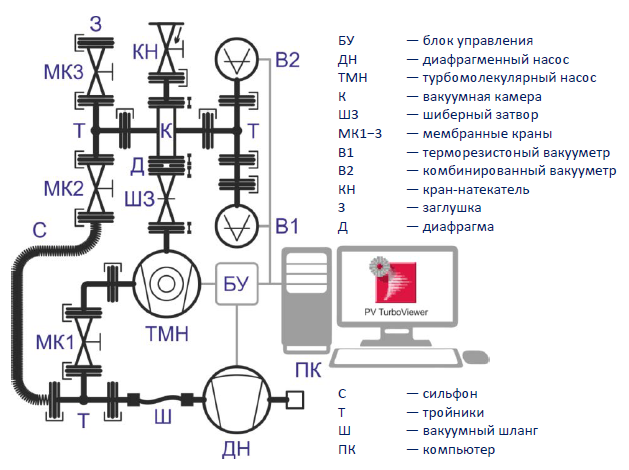
\includegraphics[width = \textwidth]{3.png}
\caption{Схема экпериментальной установки}
\label{ris3}
\end{figure}

Экспериментальный стенд выполнен на основе компактного безмасляного высоковакуумного откачного поста Pfeiffer Vacuum серии HiCube 80 Eco с диафрагменным и турбомолекулярным насосами, вакуумметров Pfeiffer Vacuum серии DigiLine, и вакуумных быстроразъёмных компонентов. Управление основными функциями откачного поста, контроль и запись параметров установки осуществляется блоком управления (БУ) через цифровой интерфейс RS-485 с помощью специального программного обеспечения PV TurboViewer8.
\begin{wrapfigure}{r}{0.3\textwidth}
	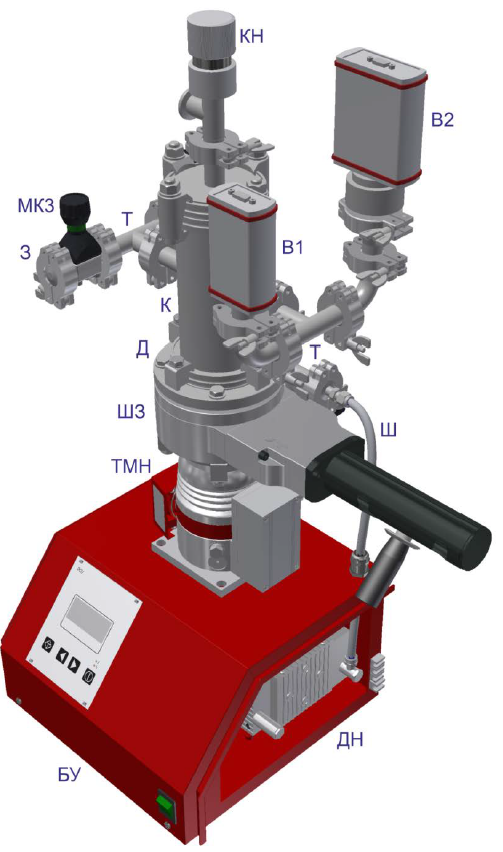
\includegraphics[width = 0.3\textwidth]{4.png}
\caption{Внешний вид экпериментальной установки}
\label{ris4}
\end{wrapfigure}
Вакуумный пост Pfeiffer Vacuum HiCube 80 Eco (PM S03 555 А) выполнен на базе диафрагменного форвакуумного насоса MVP 015 (ДН) и турбомолекулярного насоса HiPace 80 (ТМН). Откачка вакуумной камеры (К) может происходить как двумя насосами (ТМН и ДН) через шиберный затвор (ШЗ) и мембранный кран 1 (МК1), так и только форвакуумным насосом (ДН) по схеме «байпас» (англ. bypass — обходной путь), выполненной на основе вакуумных компонентов: сильфона (С), мембранного крана 2 (МК2), тройников (Т), переходников, шланга (Ш). Для контроля и измерения давления в вакуумной камере используются цифровой вакууметр PPT 100 (В1) типа Пирани (терморезисторный) и комбинированный вакуумметр MPT 100 (В2) типов Пирани (терморезисторный) и холодный катод (инвертированный магнетрон). Контролированный напуск воздушной атмосферы в камеру осуществляется через кран-натекатель EVN 116 (КН) с регулируемым потоком. Дополнительный выход с краном 3 (МК3) закрыт заглушкой (З) и служит для присоединения дополнительного объёма в случае необходимости.

\section{Используемое оборудование}

\begin{enumerate}
    \item Безмасляный высоковакуумный откачной пост Pfeiffer Vacuum;
    \item Компьютер;
\end{enumerate}

\section{Результаты измерений и обработка данных}

Начальные условия и параметры установки:

$\begin{aligned}
& P_{\text{атм}} = 760~торр\\
& V_1, V_2 = 775\pm10~см^3 \\
& \frac{L}{S} = 5,3\pm0,1~см^{-1}
\end{aligned}$\\[0,5 cm]



\section{Обсуждение результатов и выводы}


\end{document}
